% Niveau :      PCSI
% Discipline :  Elec
% Mots clés :   Elec, Ordre 2

\begin{exercise}{Condensateurs couplés}{2}{Sup}{\'Electrocinétique, Circuits d'ordre 2}{correge}

On considère le schéma suivant. Les condensateurs de même capacité $C$ sont déchargés lorsque les interrupteurs $K_1$ et $K_2$ sont ouverts.

\begin{figure}[H]
\centering
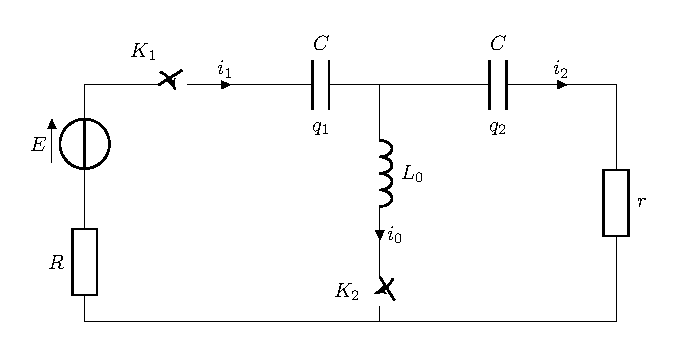
\includegraphics[scale=0.9]{elec/CondCouples.pdf}
\end{figure}

\begin{questions}

    \question En régime continu, par quels éléments peut-on remplacer condensateurs et bobines ?
    \question On ferme $K_1$, $K_2$ restant ouvert. Déterminer en un minimum de calcul  les charges $q_1$ et $q_2$ portées par les deux condensateurs identiques au bout d'un temps très long.
    \question Quelle est alors l'énergie emmagasinée par le système ? \\
              Application numérique pour $C=1\mu$F et $E=10$V.
    \question À partir de maintenant, on ferme $K_2$, $K_1$ restant fermé, et on prend une nouvelle origine des temps.
              Que vaudront l'intensité $i_0$ dans la bobine et les charges $q_1$ et $q_2$ au bout d'un temps long ? \\
              Indication : commencer par dessiner un schéma équivalent au bout d'un temps très long, et raisonner sur ce schéma à l'aide des lois de Kirchhoff.
    \question Quelles sont l'intensité $i_0$ dans la bobine et les charges $q_1$ et $q_2$ des condensateurs à $t=0^+$ ? Justifier.
    \question Écrire les lois de Kirchhoff et les lois usuelles pour les divers composants, puis établir deux équations différentielles du second ordre que vérifient les charges $q_1$ et $q_2$ des deux condensateurs après la fermeture de $K_2$.
    \question On suppose à partir d'ici que $r=R$. Montrer qu'à partir des deux équations différentielles précédentes, on obtient une équation sur $Q=q_1+q_2$ et une équation sur $q=q_1-q_2$.
    \question Résoudre ces équations, donner l'expression de $Q(t)$ et $q(t)$, et montrer en particulier que $Q$ est effectivement indépendante du temps.
    \question Les autres valeurs des composants sont prises à $L_0=5$mH, $r=200\Omega$. \\
              Montrer que 
              \[i_0(t) = \frac{r^2 C E}{16 L_0^2} t\cdot\exp\left(-\frac{r}{4L_0}t\right),\]
              et représenter graphiquement l'allure de $i_0(t)$.
\end{questions}



\end{exercise}

\begin{solution}
\begin{questions}
    \question En régime continu, une bobine est équivalente à un fil, alors qu'un condensateur est équivalent à un interrupteur ouvert.
    \question  Au bout d'un temps long, les condensateurs se comportent comme des coupe-circuits. Le courant circulant dans le circuit est donc nul. Par suite, la loi des mailles donne
                \begin{equation}
                E = u_1+u_2
                \end{equation}
                avec $u_1$ et $u_2$ les tensions aux bornes des condensateurs. Mais comme les deux condensateurs sont reliés par un fil, en régime permanent, la charge portée par leurs armatures est nécessairement la même. D'où $q_1=q_2=q$, et par suite 
                \begin{equation}
                E=2\times\frac{q}{C} \quad \Longrightarrow \quad \boxed{q = \frac{CE}{2}}
                \end{equation}
    \question On a alors l'énergie $W$ emmagasinée par le système
                \begin{equation}
                W = 2\times\frac{1}{2}\frac{q^2}{C} = \frac{CE^2}{4} = 2,5.10^{-5}J
                \end{equation}
    \question Pour un temps long, la bobine est équivalente à un fil. On a toujours $i_1=i_2=0$ car les condensateurs bloquent le courant, et par la loi des noeuds $i_0=0$. 
              En appliquant la loi des mailles dans la maille de gauche, on a $u_1=E$ (pas de tension aux bornes des résistances), donc $q_1=CE$. Dans la maille de droite, $u_2=0$ donc $q_2=0$.
    \question Par continuité de l'intensité traversant une bobine, $i_0(0^+)=0$. Par ailleurs, la charge au borne d'un condensateur est une fonction continue (car la tension l'est), donc on a $q_1(0^+)=q_2(0^+)=\frac{CE}{2}$.
    \question On écrit la loi des mailles dans les mailles de droite et de gauche :
                \begin{align}
                    E &= u_0+u_1+Ri_1 \\
                    0 &= u_0-u_2-ri_2
                \end{align}
                On a bien sûr $i_1=i_0+i_2$. 
                Par ailleurs, $u_1 = \frac{q_1}{C}, u_2=\frac{q_2}{C}$, et finalement:
                \begin{equation}
                    u_0=L_0\dv{i_0}{t}=L_0\dv{(i_1-i_2)}{t} = L_0\left(\dv{ q_1}{t}-\dv{q_2}{t}\right).
                \end{equation}
                En réarrangeant les équations de mailles, on obtient donc les équations différentielles couplées

                \begin{equation}
                \label{eqcouple}
                \boxed{
                \left\{\begin{array}{ll}
                \dv{ q_1}{t}-\dv{ q_2}{t}+\frac{R}{L_0}\dv{q_1}{t}+\frac{q_1}{L_0 C} = \frac{E}{L_0}\\
                \dv{q_1}{t}-\dv{ q_2}{t}-\frac{r}{L_0}\dv{q_2}{t}-\frac{q_2}{L_0 C} = 0 \\
                \end{array}\right.}
                \end{equation}
    \question  Les équations présentées ici sont caractéristiques de ce qu'on appelle des modes symétriques et antisymétriques (vous les retrouverez en TP lors de l'étude des pendules couplés). L'astuce habituelle pour les découpler consiste à faire apparaître les combinaisons $Q=q_1+q_2$ et $q=q_1-q_2$. Puis, prenant (\ref{eqcouple}), et calculant la somme et la différence des deux équations, on obtient finalement

                \begin{equation}
                \boxed{ \left\{\begin{array}{ll}
                    \dv{q}{t}+\frac{r}{2L_0}\dv{q}{t}+\frac{q}{2L_0 C} = \frac{E}{2L_0} \\
                    \dv{Q}{t}+\frac{Q}{rC} = \frac{E}{r} 
                \end{array}\right.}
                \end{equation}
    \question Résolvons l'équation différentielle pour $Q$. Il s'agit d'une équation différentielle du premier ordre avec second membre. La solution de l'équation homogène associée est $Q_H(t) = Ke^{-t/rC}$. Une solution particulière est $Q_p(t) = CE$. La condition initiale est 

                \begin{equation}
                Q(0) = q_1(0)+q_2(0) = CE \Rightarrow K+CE = CE \Rightarrow K=0 !
                \end{equation}

                Ainsi, $\boxed{Q(t)=CE=\text{cste}}$ : la charge totale des deux condensateurs reste constante.

                On résout maintenant l'équation différentielle associée à $q$. Il s'agit d'une équation du second ordre. On commence par résoudre l'équation sans second membre. L'équation caractéristique est
                \[x^2+\frac{r}{2L_0}x+\frac{1}{2L_0C}=0.\]

                Son discriminant vaut $\Delta = \frac{r^2}{4L_0^2}-\frac{2}{L_0C} \approx 0$ avec le degré de précision des données du problème. On a donc une racine double $x=\frac{r}{4L_0}$, et la solution se met sous la forme $q_H(t) = (At+B)\exp\left(-\frac{r}{4L_0}t\right)$. Une solution particulière étant $q_p(t)=CE$, on a alors 

                \begin{equation}
                q(t) = CE+(At+B)\exp\left(-\frac{r}{4L_0}t\right).
                \end{equation}

                Les conditions initiales sont $q(0^+) = q_1(0^+)-q_2(0^+) = 0$, ce qui amène $B=-CE$. Par ailleurs, $\dv{q}{t}(0^+) = \dv{q_1}{t}(0^+)-\dv{q_2}{t}(0^+) = i_1(0^+)-i_2(0^+) = i_0(0^+) = 0$, et $\dv{q}{t} = (A-\frac{r}{4L_0}(At-CE))\exp\left(-\frac{r}{4L_0}t\right) = A+\frac{rCE}{4L_0}$, soit $A=-\frac{rCE}{4L_0}$. Finalement 

                \begin{equation}
                q(t) = CE\left(1-(1+\frac{r}{4L_0}t)e^{-\frac{r}{4L_0}t}\right).
                \end{equation}
    \question On sait que $i_0 = i_1-i_2$, donc $i_0=\dv{q}{t}$, ce qui donne
                \begin{equation}
                    i_0(t)=CE\left(-\frac{r}{4L_0}+\frac{r}{4L_0}(1+\frac{r}{4L_0})\right)\exp(-\frac{r}{4L_0}t)
                \end{equation}
                \begin{equation}
                \boxed{i_0(t) =\frac{r^2CE}{16L_0^2}t.\exp\left(-\frac{r}{4L_0}t\right)}
                \end{equation}
\end{questions}

\end{solution}